\documentclass{beamer}
\title[Continuous Descent Approach \hspace{2em}\insertframenumber/\inserttotalframenumber]{Continuous Descent Approach (CDA)}
\subtitle{Benefits and Challenges}
\author{Christopher Ngigi}
\date{April 16, 2015}
\usetheme{Warsaw}
\usepackage[version=3]{mhchem}
%\usepackage{caption}
\begin{document}

\addtocounter{framenumber}{-1}

\frame{\titlepage}


%%==============================================

\begin{frame}
\frametitle{Motivation for CDA}

{\color{blue} Background}
\begin{enumerate}[1.]
\item Aircraft as a source of pollution. 

\begin{figure}[h!]
\centering
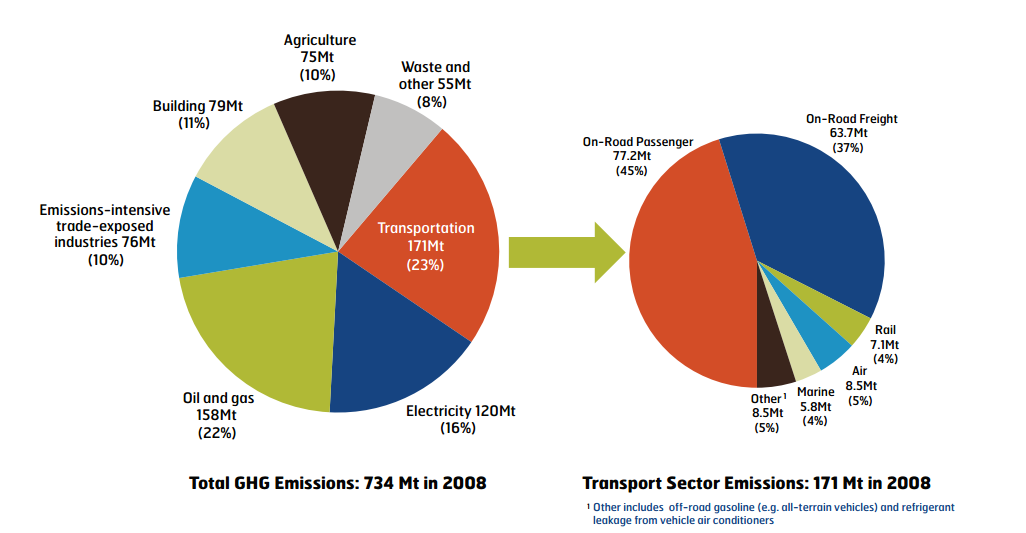
\includegraphics[width=0.9\textwidth]{./figures/TotalEmissions.png}\\
{\tiny Aviation's contribution to greenhouse gas emissions [Transport Canada 2012]}
\end{figure}
\end{enumerate}

\end{frame}

%%==============================================


\begin{frame}
\frametitle{Aviation emissions}
\begin{enumerate}[1.]
\setcounter{enumi}{1}
\item Growing trend in pax numbers
\item Fuel emissions: long-term effects
\begin{itemize}
\item Radiative Forcing (RF) = change in energy in the atmosphere due to GHG emissions.
\item $NO_x$ $\rightarrow$ short duration life: 2 weeks life-cycle
\item $CO_2$, $\rightarrow$ life-cycle of $\approx$ 150-200 years. Can lead to acid rain.
\item AIC: differing opinions on scale of aviation induced cirrus (AIC) effects. The tiny ice crystals absorb thermal radiation in the upper atmosphere: overall warming effect (RF)
\end{itemize}

\item Will focus on direct fuel emissions, and not AIC.
\item Time to develop for radical situation-changing designs $>>$ time we have available
\end{enumerate} 

\end{frame}


%%==============================================

\begin{frame}
\frametitle{Continuous Descent Approach}

\begin{enumerate}[1.]
%\setcounter{enumi}{1}
\item Reducing fuel consumption will cut back emissions
\item CDA : aircraft descends smoothly from cruise alt to runway, no "steps" of intermittent level segments


\begin{figure}[h!]
\centering
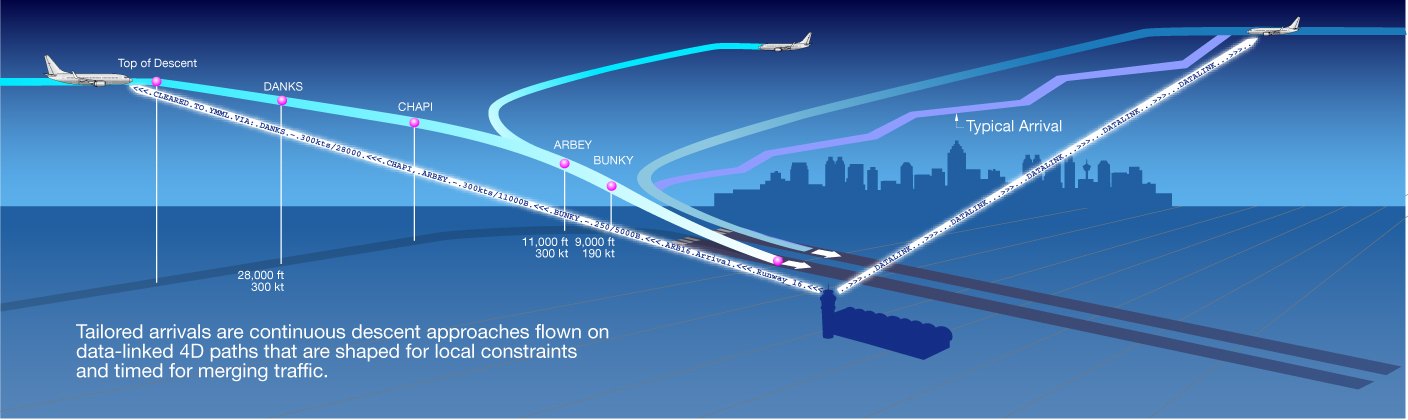
\includegraphics[width=1\textwidth]{./figures/Tailored_Arrivals_YMML.jpg}\\
{\tiny {Tailored arrivals into Melbourne Intl [Boeing 2009]}}
\end{figure}

\item Started at Heathrow in the $70s$ to reduce noise. From $7000ft$

\item Significant promise : (during landing phase) reducing fuel consumption, emission, noise impact and flight time.

\end{enumerate}

\end{frame}

%%============================================================================

\begin{frame}
\frametitle{Benchmark scenario}

\begin{enumerate}[1]

\item ANZ and QANTAS participated in the Aspire program.  Goal was set ideal flight benchmark metric in maximum savings.

\item Framework: 
\begin{itemize}
\item ANZ-operated Boeing 777, Auckland - San Francisco. September 2008.
\item Most advanced air navigation available
\item Practically, all operational restraints removed:  ATC: (congestion control vectoring, fixed route structure, procedures, flow restrictions) and airline restraints. 
\end{itemize}

\item Achieved \textbf{3.5} tonnes fuel savings (\textbf{11.2} tonnes CO 2 reduction). 
\item One month later Qantas. New A380 from KLAX -YMML. Saving \textbf{8.9} tonnes fuel (\textbf{28} tonnes $CO_2$ ). 
\item CDA contributed to these savings
\end{enumerate}

\end{frame}



%=============================================================================

\begin{frame}
\frametitle{Literature review}

\begin{enumerate}[1]

\item Some literature researching the effects of CDA was analyzed.

\item 50\% was from an academic setting, the rest from institutions

\item Using radar databases from airports:

\begin{itemize}
\item used for optimization model development; 
\item algorithms for traffic decongestion: FMC and ground support systems
\end{itemize}

\item Data from flights:

\begin{itemize}
\item ATC/Crew communication simulations
\item Model infrastructure to support decision making
\end{itemize}

\end{enumerate}

\end{frame}



%==============================================================================

\begin{frame}
\frametitle{Results: Benefits}

Benefits of implementing CDA:
\begin{enumerate}[1.]

\item Fuel savings:
\begin{itemize}
\item While descent/landing does not contribute to significant fuel usage, CDA has been proven to save fuel.	
\item Actual figures vary for single-aisle and twin-aisles
\item Cao et al [2013] found on average, arrivals into KATL saved $\approx$ 160kg fuel/flight 
\item Having a direct descend without level segments allows sustained near-idle engine runs with minimal throttle-ups 
\item level segments have enforced speed restrictions $\rightarrow$ slowing the plane at constant altitude
\item Only valid for optimized CDA profiles (routing, weather)
\end{itemize}
\end{enumerate}
\end{frame}


%=================================================================

\begin{frame}
\frametitle{Results: Benefits - cont'd}
\begin{figure}[h!]
\centering
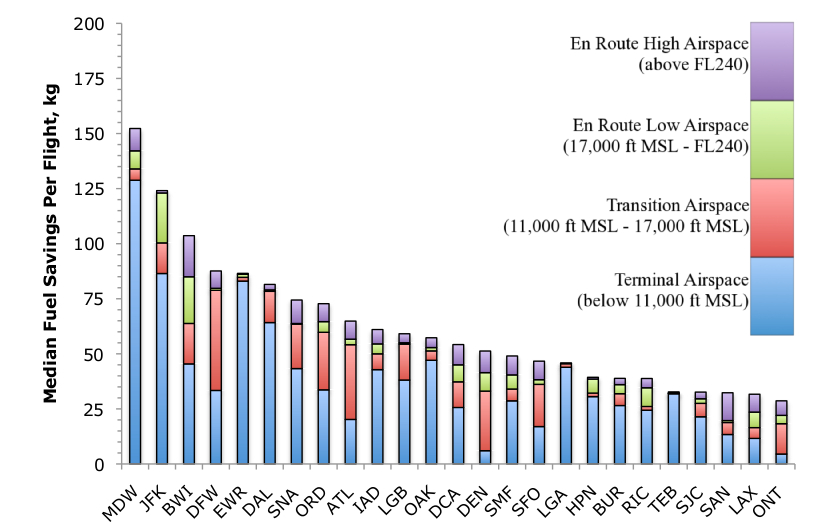
\includegraphics[width=0.8\textwidth]{./figures/Comparison.jpg}\\
{\tiny Effect of continuous descent scenario on median fuel savings by airport [Robinson and Kamgarpur 2010]}
\end{figure}
\end{frame}


%===================================================================

\begin{frame}
\frametitle{Results: Benefits - cont'd}

\begin{enumerate}[1.]
\setcounter{enumi}{1}
\item Reduction in emissions:
\begin{itemize}
\item Reduction in fuel corresponds to lower fuel-based emissions
\item Coppenbarger et al [2007] (Study on B777 trans-Pacific flights) found CDA could reduce $CO_2$ emissions by as much as 350 kg/flight depending on traffic conditions. 12\% reduction in $NO_x$ (Alam et al [2010])

\item Significant noise reduction (Alam and co-authors [2010]) in vicinity of airport along the descent flightpath due to virtual elimination of extended level segments

\end{itemize}

\item Time savings: approximately 2min (Turgut et al [2010]). A small figure, although when compounded could relate to significant savings in direct operating costs (DOCs) - salaries, maintanance, fees.


\end{enumerate}

\end{frame}



%==============================================================================

\begin{frame}
\frametitle{Results: Drawbacks}

\begin{enumerate}[1.]
%\setcounter{enumi}{1}
\item Level of automation: detailed support infrastructure required

\begin{figure}[h!]
\centering
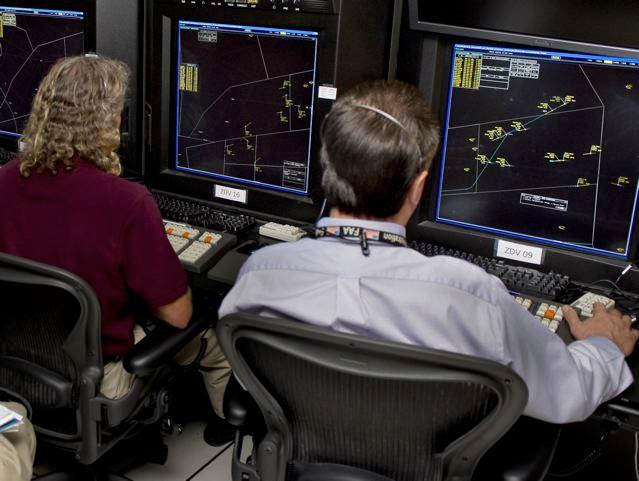
\includegraphics[width=0.7\textwidth]{./figures/EDA.jpg}\\
{\tiny Efficient Descent Advisor (EDA), a decision-support tool for air-traffic controllers managing arrival airspace in enroute facilities [Coppenbarger et al 2010]}
\end{figure}

\end{enumerate}
\end{frame}

%===================================================================

\begin{frame}
\frametitle{Results: Drawbacks - cont'd}

\begin{enumerate}[1.]
\setcounter{enumi}{1}
\item Information flux. Crossflow between ATC and the pilot/FMS via datalink. Safety.
\item Plenty of benefits of CDA are curtailed by heavy traffic conditions
\item Complexity: CDA inadvertently provides aircraft with descent trajectory self-autonomy. The system is harder to control.
\item Poorly designed CDAs can lead to more traffic conflict, fuel usage
\item Heavy capital cost of support infrastructure
\item Additional training for crew and ATC. Long-established routines difficult to adjust.

\end{enumerate}

\end{frame}


%=========================================================================

\begin{frame}
\frametitle{Results: Observations}

\begin{enumerate}[1.]
\item CDAs can be optimized for criteria: minimal fuel burn, flight time
\item CDA easiest to implement in low traffic conditions

\begin{figure}[h!]
\centering
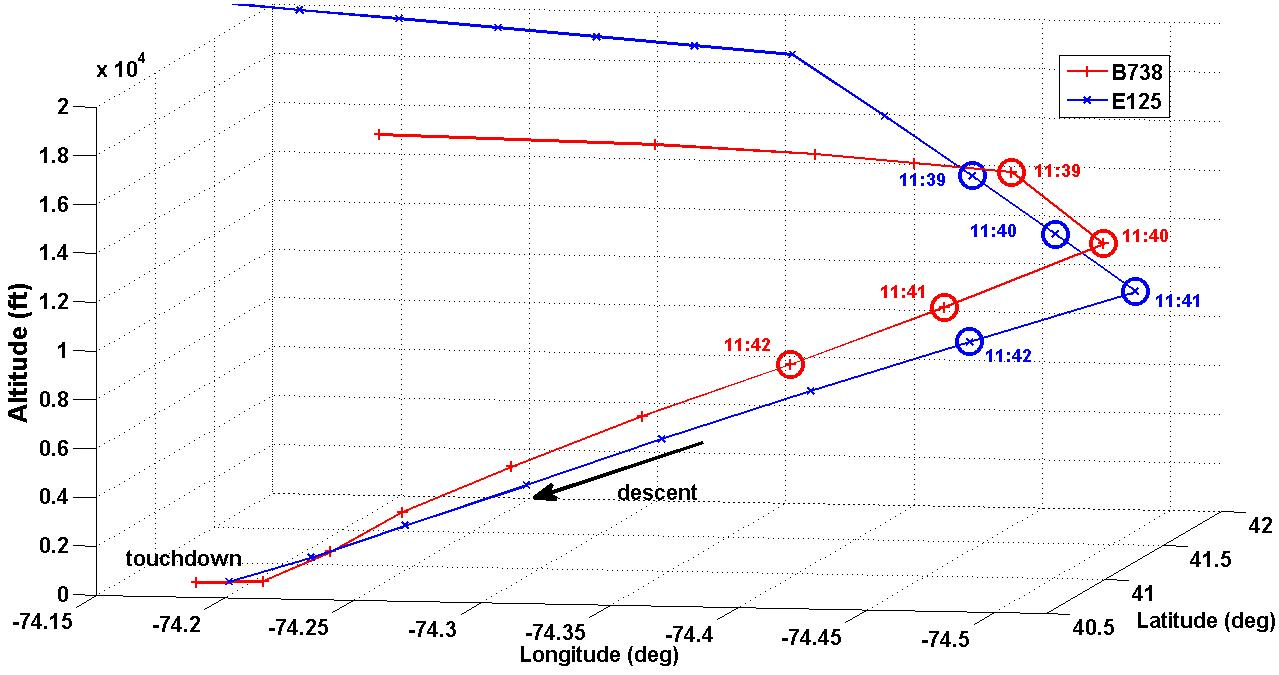
\includegraphics[width=0.8\textwidth]{./figures/reschedule.jpg}\\
{\tiny Two aircraft in conflict get rescheduled [Cao et al 2011]}

\end{figure}
\end{enumerate}
\end{frame}

%=====================================================================

\begin{frame}
\frametitle{Results: Observations - cont'd}

\begin{enumerate}[1.]
\setcounter{enumi}{1}
\item Although individual flights fail to achieve fuel savings, airport as a whole realizes fuel savings.
\item Fuel burn=$f($altitude, speed$)$ - sustain high alt as long as possible to realize max savings.
\item System automation has great promise to reduce information overload. (ATC/Crew)
\item Due to their long flights, wide-bodies are greatest beneficiaries of CDA - high priority. More could be done about single-aisle; they account for bulk traffic movement.
\item Time restrictions could reduce fuel savings.

\end{enumerate}

\end{frame}
%======================================================

\begin{frame}
\begin{center}
{\huge Thank You For Your Attention!} \\
\vspace*{1.5cm}
{\Large Questions?}
\end{center}

\end{frame}

%%==============================================
\appendix
\newcounter{finalframe}
\setcounter{finalframe}{\value{framenumber}}

\setcounter{framenumber}{\value{finalframe}}
\end{document}